% !TeX spellcheck = en_US

\chapter{Overall component-based software development process}
\label{chap: Software development process}
\section{Introduction}
In this chapter the design and implementation steps for the component-based software engineering (CBSE) approach are elaborated. The software design process involves two main actors: the software architect who is responsible for the entire software and provides support at system-level to the customer, and the software supplier who is responsible for the development of part of the software \cite{CompBasedProcess}. The parts of the software supplied by the software suppliers are then integrated in the final integration step.

Most of the activities described below come under the responsibility of the software architect, but as soon as the component is defined, it can undergo a detailed design and code implementation. This may indicate some shortcomings and flaws in the design of the component, which might trigger a re-design, re-negotiation of the component definition. This often leads to an iterative/incremental development process \cite{ScheduAnaly}. Detailed design and implementation of components are usually done by the software developers or it may be subcontracted to third party software suppliers. 

\section{Design entities and design steps}
\label{section: Design steps}
There are two kind of entities which are defined in OSRA: Design-level entities which are explicitly specified in the design space and require the skills of the user to use them, real-time architecture entities which are not explicitly represented in the design space, instead they are automatically generated by the code-generation engines. The automatic generation of containers and connectors are possible only upon the knowledge of the computation model and execution platform that are going to be adopted \cite{SAVOIR}\cite{CompBasedProcess}. As already mentioned in the previous chapter, this master thesis considers Tasking Framework as the computational model and a normal linux based PC as the execution platform.   

The following entities belong to the design space: Data types, events, interfaces, component types, component implementations, component instances, component bindings and the entities required for the description of the hardware topology and platforms. The following entities belong to the real-time architecture: containers and connectors.

The development process is clearly divided into different steps \cite{CompBasedProcess}\cite{PhdThesis}\cite{SAVOIR}:

\begin{description}
\item [Step 1: Definition of data types and events] Data types are the basic entities in the approach and they can be primitive types, enumerations, ranged or constrained types, arrays or composite types (like structs in C or record types in Ada). An event is used in the publish-subscribe communication paradigm and it is an asynchronous message passing scheme. 

\item [Step 2: Definition of interfaces] A set of operations with one or more already typed parameters, each with a direction (\texttt{in, in out, out}) are grouped together to form an interface. The interface can also hold a set of interface attributes of an already defined data type. The interface attributes can have read-only or read-write accesses. From the list of interface attributes, set of \texttt{getter} and \texttt{setter} operations can be generated for the attribute access, in particular \texttt{getter} operations for attributes with \texttt{read} only access and \texttt{getter} and \texttt{setter} operations for attributes with \texttt{read-write} access. 

\cref{fig: Datatypes events and interfaces} depicts three data types and an event. Interfaces \texttt{AOCS\_IF} and \texttt{THR\_IF} implement only operations while interface \texttt{GYR\_IF} comprises one read-only attribute.

\begin{figure}[h]
	\centering
	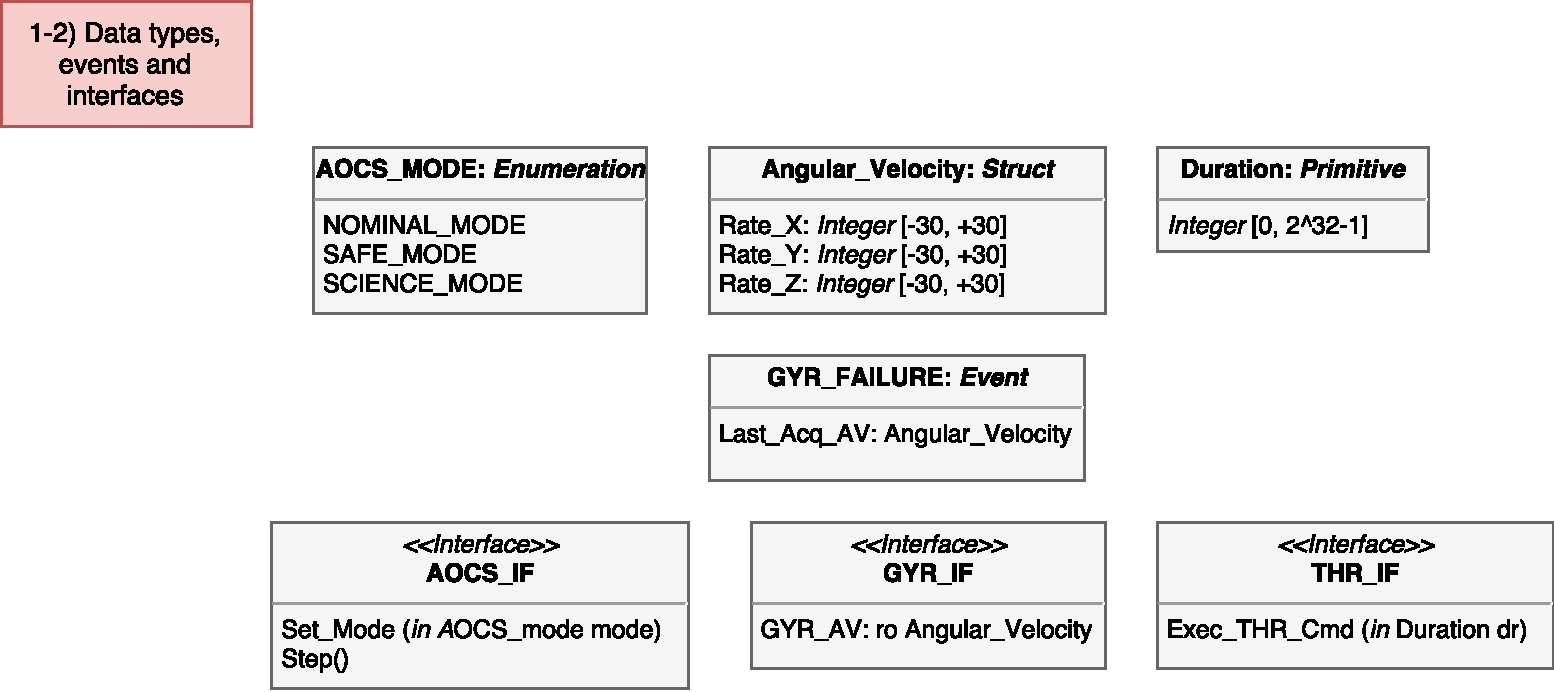
\includegraphics[width=0.8\textwidth]{DatatypesEventsInterfaces.pdf}
	\caption{Data types, events and interfaces}
	\source{\cite{CompBasedProcess}}
	\label{fig: Datatypes events and interfaces}
\end{figure}

\item [Step 3: Definition of component types] Component types form the basis of a reusable software asset \cite{CompBasedProcess}. The software architect defines the component type to provide the specification of the functions that the component of the respective type would implement. The component types are independent of each other and they can consist of:
\begin{itemize}
\item One or more provided interfaces, which list the services that the component of the respective type would provide.
\item One or more required interfaces, which list the functional services that the component of the respective type would require in order to function correctly according to the functional specifications.
\item A set of component type attributes of already defined data types that are local to the component and cannot be accessed from outside.
\item Event emitter/receiver ports to raise or receive events.
\end{itemize}

In order to specify the provided and required interfaces, the component type references the interfaces that were defined in Step 2. This helps in straight forward matching of the required and provided interfaces.  

\cref{fig: Component type} depicts a component type \texttt{AOCS}. This component type provides interface \texttt{AOCS\_IF} and requires interfaces \texttt{GYR\_IF} and \texttt{THR\_IF}. It also raises events of type \texttt{GYR\_FAILURE}. 

\begin{figure}[h]
	\centering
	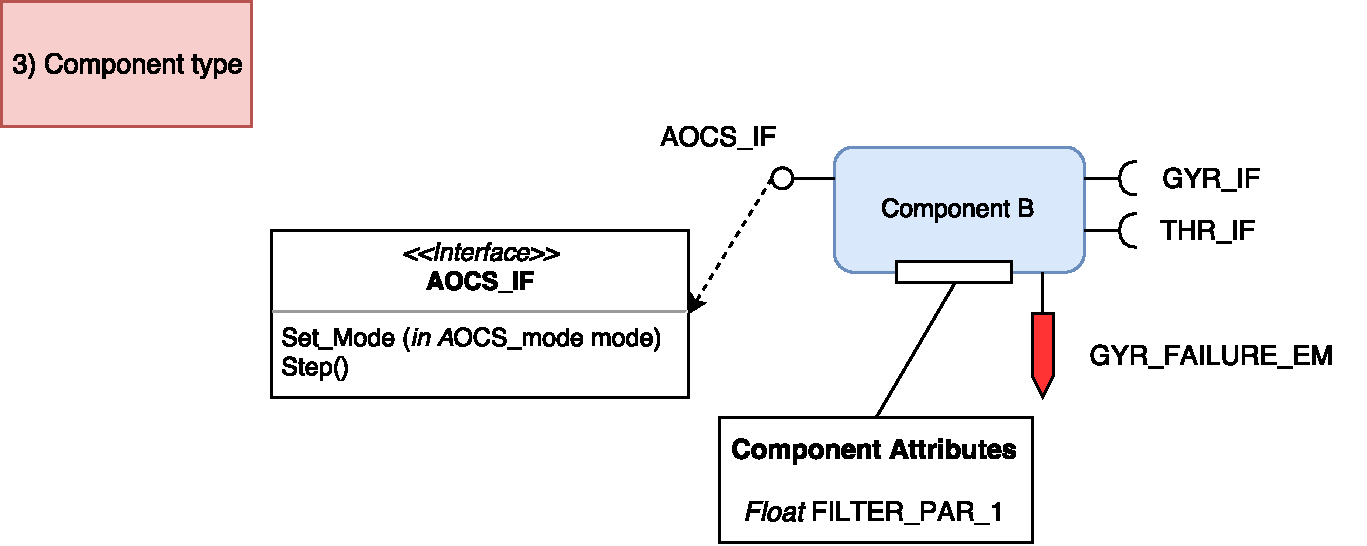
\includegraphics[width=0.8\textwidth]{ComponentType.pdf}
	\caption{Component type}
	\source{\cite{CompBasedProcess}}
	\label{fig: Component type}
\end{figure}

\item [Step 4: Definition of component implementations] The software architect can create and refine a component implementation from the component type. The component implementation contains the functional code in the form of source code that implements all the services that the component is supposed to provide. It acts as a  black box and only its external interfaces are only that matter. It is also a subcontracting unit to the software supplier. 

A component type can have more than one implementation and all of these implementations contain only pure sequential code i.e. it is void of any tasking or timing constructs. Implementations can be developed in multiple languages such as Ada, C, C++ etc.  

The component implementation should also provide constructs to store the attributes exposed through its provided interfaces and its component type. Technical budgets such as \ac{wcet} for a particular operation, maximum memory foot-print for component implementation, maximum number of calls to a certain operation on a required interface, can be placed on the entire component or on the operations and the implementation of the component shall respect this budget. Despite a sequential nature of the code, a component implementation may set specific non-functional constraints to preserve the functional correctness of its behavior. Component implementation is thus a particularly attractive unit to be subcontracted to a third-party software supplier because the software architect can define components, attach technical budgets to it and delegate the implementation to he software suppliers. The software suppliers might add additional operations to the component implementation as and when necessary for the implementation \cite{CompBasedProcess}. 

\cref{fig: Component implementation} depicts one of the many possible component implementations for the component type \texttt{AOCS}.

\begin{figure}[h]
	\centering
	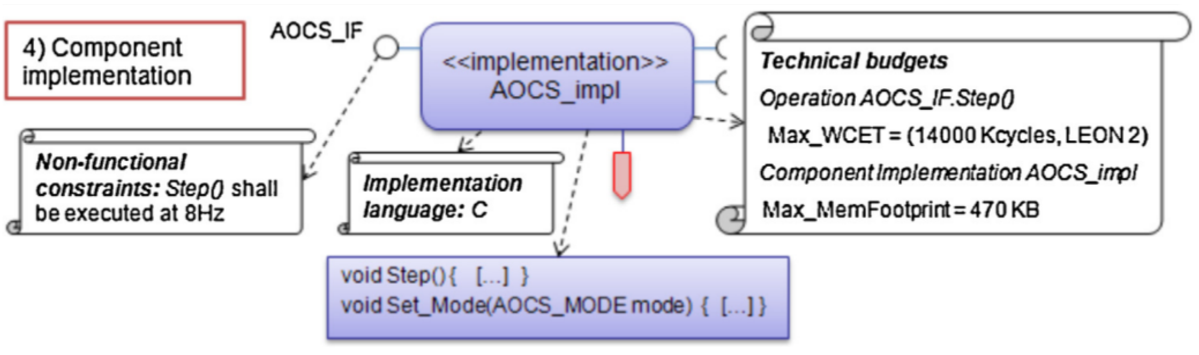
\includegraphics[width=0.8\textwidth]{ComponentImplementation.pdf}
	\caption{Component Implementation}
	\source{\cite{CompBasedProcess}}
	\label{fig: Component implementation}
\end{figure} 

\item [Step 5: Definition of component instances] A component instance is an instance of a component implementation. It is a deployment unit which is subjected to allocation on a processing unit and it is an entity on which the non-functional properties are specified. Specifically, the non-functional properties are attached, as in \cref{fig: Component instances}, to the provided interface side of the component, as they are the expression of a property or a provision of the component instance.

\item [Step 6: Definition of component bindings] Component bindings, as the name suggests, are the connections between one required interface of a component and the provided interface of another component. These bindings are set at design time and is subjected to static type matching to ensure that correct required and provided interfaces are connected to one another. This can be done by asserting the compatibility of the two interfaces (by type system or by inspection of the signature of their operations). If the binding is legal then whenever a call is made to an operation in the required interface, the call is dispatched to the correct operation in the bound provided interface. The signature of the calling operation in the \ac{ri} and the called operation in the \ac{pi} are different and the connector, connecting these two interfaces, is in charge of performing this step. A tool support (possibly a back-end code generator) should initiate the configuration of the connector to perform this kind of binding.

It is also possible in this step to define bindings between an event emitter port of one component and an event receiver port of another component as shown in \cref{fig: Component instances}.

\item [Step 7: Specification of non-functional attributes] After component instances and component bindings have been defined, the software architect can add non-functional attributes to the services of the provided interfaces. 

In this step, the software architect specifies the timing and the synchronization attributes \cite{CompBasedProcess}. At first, the concurrency kind of the operation is established, and they can be \texttt{synchronous} or \texttt{asynchronous} operations. In case of a \texttt{synchronous} operation, it is executed in the flow of control of the caller and in case of an \texttt{asynchronous} operation, the operation is executed by a dedicated flow of control on the side of the callee. 

A \texttt{synchronous} operation is said to be \texttt{protected} if it needs to be protected from data races in case of concurrent calls. The operation is said to be \texttt{unprotected} if it is free from such risks. In case of a \texttt{asynchronous} operation type, the architect can choose one of the following release patterns for the operation:

\begin{description}
\item [Periodic operation] The execution platform executes the operation at fixed periods with a dedicated flow of control.
\item [Sporadic operation] Two subsequent execution requests are separated by a minimum timespan called the \ac{miat}. The execution platform and the infrastructural code should guarantee this MIAT separation between two subsequent calls to the operation and the component implementer does not have to worry about it.
\item [Bursty operation] Only particular number of activations of an operation is allowed in a bounded interval of time. Again, as in the case for sporadic operation, the execution platform and the infrastructure code guarantees this and the component implementer does not have to worry about it.
\end{description} 

For all the operations which have concurrency kind set as \texttt{asynchronous}, the software architect must provide the worst case execution time (WCET) of the operation. A preliminary value of WCET is initially provided based on previous use of operations in other projects (if any) and they can be refined with bounds at later stages after performing a timing analysis for a given target platform.

\cref{fig: Component instances} depicts the component bindings between the required and provided interfaces of the \texttt{AOCS} and \texttt{Mode\_Manager} component instances. It also depicts the non-functional properties which are specified on the services provided by the provided interfaces.

\begin{figure}[h]
	\centering
	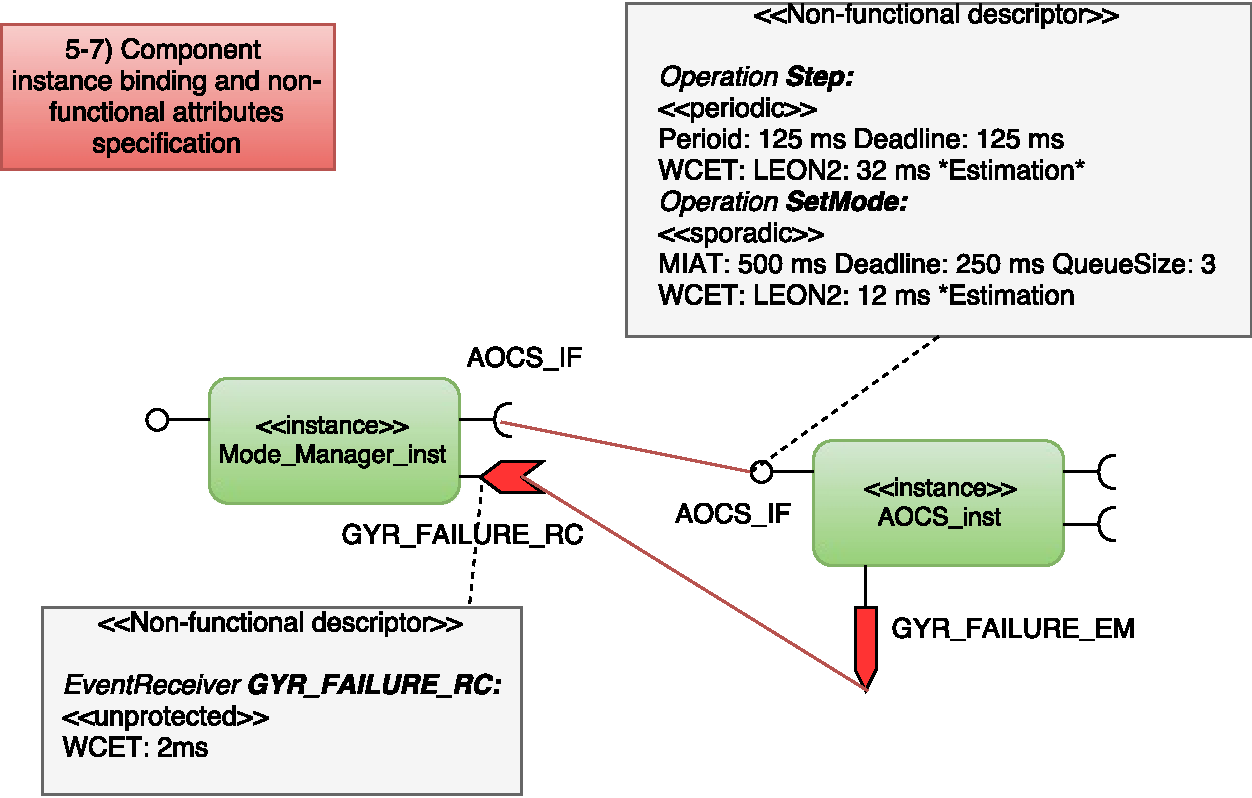
\includegraphics[width=0.8\textwidth]{ComponentInstances.pdf}
	\caption{Component instance, component bindings and decoration with non-functional attributes}
	\source{\cite{CompBasedProcess}}
	\label{fig: Component instances}
\end{figure}

\item [Step 8: Definition of physical architecture] The hardware topology provides a description of the system hardware limited to the aspects related to communication, analysis and code generation. It also provides a model-level description of the relevant hardware of the system. In the hardware topology, following elements are described:
\begin{itemize}
\item Processing units that have a general-purpose processing capability.
\item Avionics Equipment/Instruments/Remote terminals.
\item The interconnection between the elements mentioned above. 
\item A representation of the ground segment/other satellites (eg. Formation flying) to state the connection between the satellite and ground segment or other space segments.
\end{itemize}		
For the specification of these elements, following attributes are used:
\begin{description}
\item [Processor frequency] This is used for processors to re-scale WCET values expressed in processor cycles in Step 6.
\item [Bandwidth] This is used for buses and point-to-point links and it indicates maximum blocking time due to non-preemptability of the lower priority message transmission (for whatever reason), minimum and maximum size of packets, minimum and maximum propagation delay, maximum time that the bus arbiter/driver needs to prepare and send a message on the physical channel and maximum time for the message to reach the receiver.    
\end{description}

\item [Step 9: Component instances and component bindings deployment] In this step, the component instances are allocated on the processing units defined in the hardware topology in Step 8. In majority of the cases, it is straight-forward to allocate the bindings between the components because they are deployed on the same processing units \cite{CompBasedProcess}. In other cases, they need to be specifically allocated.

\item [Step 10: Model-based analysis] The system model developed within the software reference architecture is subjected to schedulability analysis to determine whether the timing requirements set in the interfaces can be met.

From the user model which is a \ac{pim}, a \ac{sam}, which is a \ac{psm} is created. This model is subjected to analysis and the results of the analysis is available for the software architect as a read-only result. 

The analysis transformation chain requires a model representation of the generated containers and connectors to be defined in the SAM for an accurate analysis \cite{CompBasedProcess}.

Please note that, step 10 is not of concern in this Master thesis as this Master thesis deals only with automatic generation of containers and connectors and hence an accurate model based schedulability analysis is outside the scope. It is assumed in this Master thesis, that the user models successfully pass the Model based schedulability analysis and hence are  subjected directly to the model-code transformation. The actual flow is as depicted in \cref{fig: Automatic code generation}. Also, Steps 8-9 are not of concern in this Master thesis, as it deals with hardware modeling and they are again outside the current scope of this Master thesis. However, these steps were mentioned for the sake of clarity and continuity.

\begin{figure}[h]
	\centering
	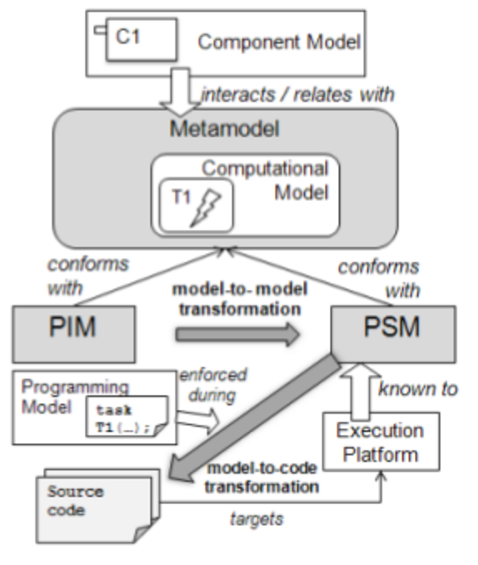
\includegraphics[width=0.4\textwidth]{AutomaticCodeGeneration.pdf}
	\caption{Generation of SAM and model-code transformation}
	\source{\cite{CompBasedDev}}
	\label{fig: Automatic code generation}
\end{figure}

\item [Step 11: Generation of containers and connectors]  This step is one of the main focus points of this Master thesis as mentioned before. Containers and connectors are generated and they specify:
\begin{itemize}
\item The structure of each container in terms of the required and provided interfaces of the enclosed component that they delegate and subsume.
\item The structure of each connector. 
\end{itemize} 
The non-functional attributes, component instances deployment and component connectors deployment play a major role in determining the creation of connectors and containers and how component instances and their operations are allocated to them.

Concurrency can be achieved by encapsulating sequential procedures into tasks which reside in containers and the protection from concurrent accesses can be provided by attaching them concurrency control structures. All of this can be achieved without modifying he sequential code and simply by following the use relations among the components.

In order for the OBSW to interact with the external world, sensors and actuators need to be provided. These hardware entities are represented as pseudo components (A pseudo-component indicates that a component is for interaction purposes only) and software capability is attached to these components at the component instance level.    
\end{description}

\cref{fig: Containers} depicts the automatic generation of containers and connectors for the components \texttt{AOCS} and \texttt{Mode\_Manager}. It also shows how their component instances are allocated to them. 

\begin{figure}[h]
	\centering
	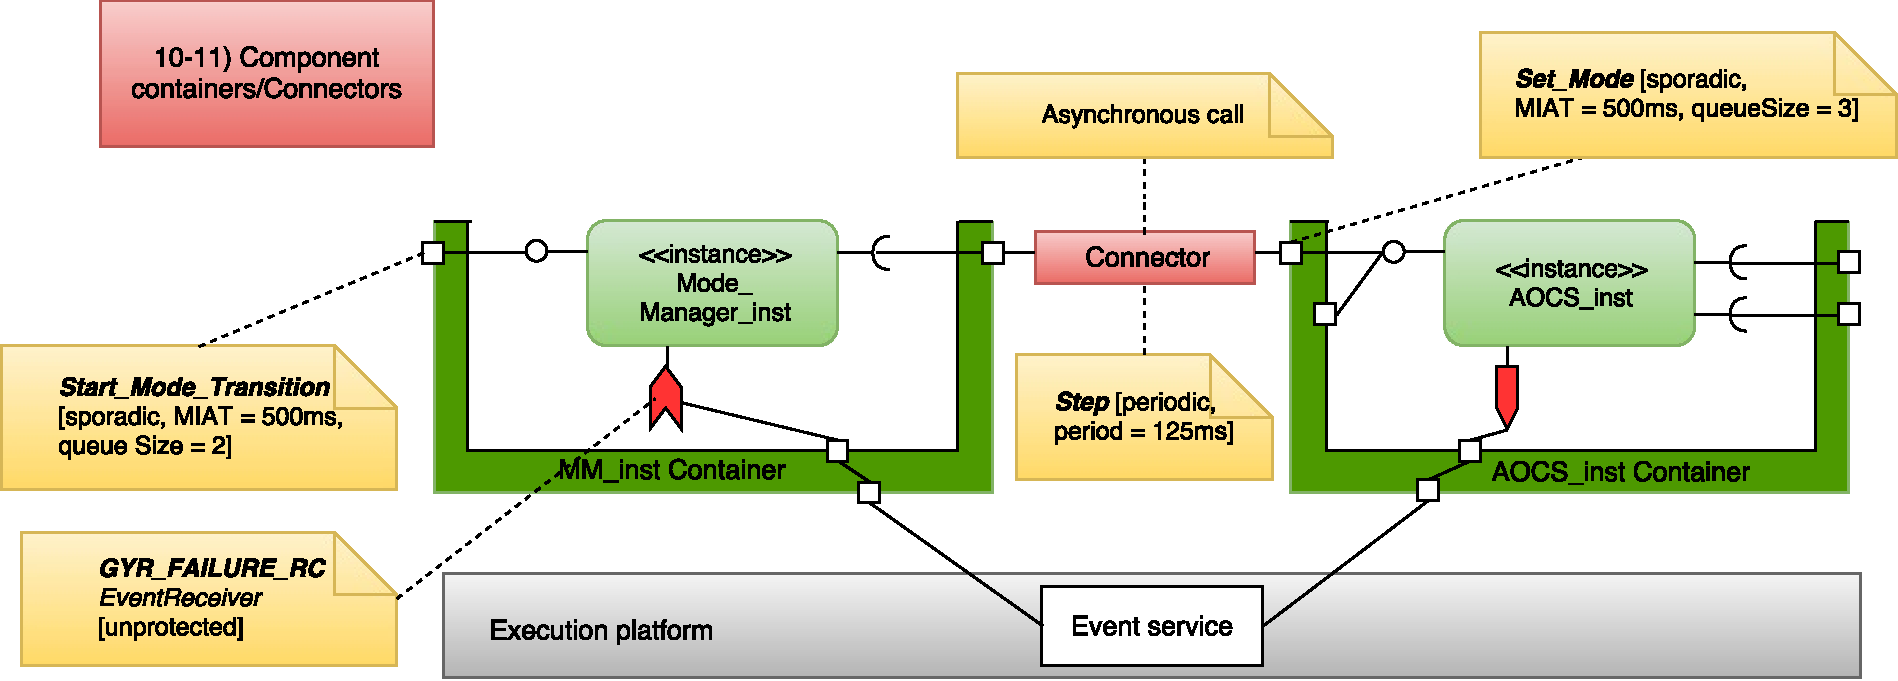
\includegraphics[width=1.0\textwidth]{Containers.pdf}
	\caption{Automated generation of containers and connectors}
	\source{\cite{CompBasedProcess}}
	\label{fig: Containers}
\end{figure}

\section{Design flow and design views}
\label{section: Design flow and views}
When the component model is defined, it also defines implicitly a design flow as shown in \cref{fig: Design flow}, that needs to be followed, to be able to create an OBSW that meet all of its user needs and high level requirements \cite{SAVOIR}\cite{PhdThesis}\cite{CompBasedProcess}. The design flow is as explained in the previous section. 

\begin{figure}[h]
	\centering
	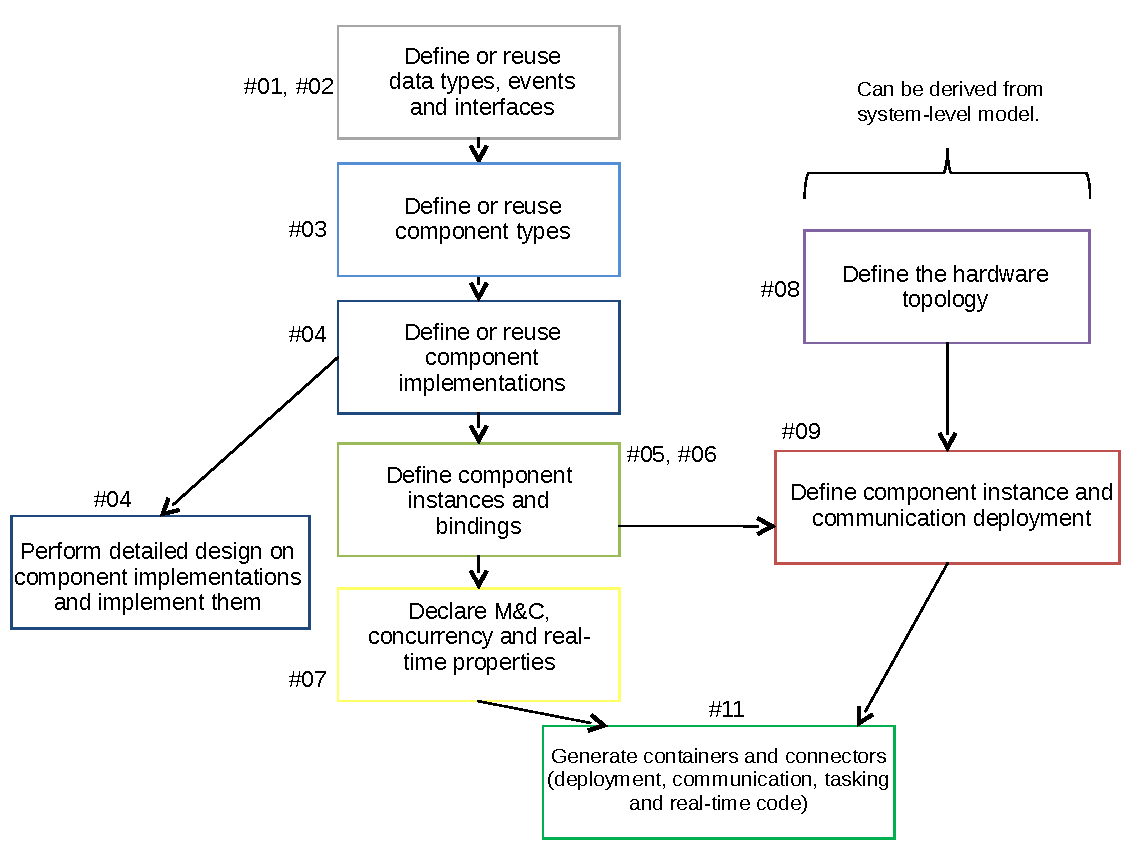
\includegraphics[width=0.8\textwidth]{OverallFlow.pdf}
	\caption{The overall design flow}
	\label{fig: Design flow}
\end{figure}

The Obeo Designer Framework \cite{obeoDesigner} provides a concept called 'Viewpoint' and using this concept, the design views are implemented \cite{CompBasedProcess}. One of the advantages of the design views is to promote or enforce a certain design flow \cite{CompBasedProcess}. The component model is accompanied by the following design views:
\begin{description}
\item [Data view] This view is for the description of data types and events.
\item [Component view] For definition of interfaces, components and the binding between them to fulfill their required needs.
\item [Hardware view] For the specification of the hardware and the network topology.
\item [Deployment view] For the allocation of components to computational nodes.
\item [Non-functional view] In this view, the non-functional attributes are attached to the functional description of components.
\item [Space-specific view] In this view, the services related to the commandability and observability of the spacecraft are specified.
\end{description}  

\section{Language units of the OSRA}
\label{Language units}
The modeling language provided to the software architect to model the OBSW is divided for the ease of construction of the OBSW models into a set of language units \cite{SpecMetamodel}. Each language unit consists of closely related metamodel entities. The language units are grouped into separate meta-models for the sake of re-use as shown in \cref{fig: Language units} \cite{SpecMetamodel}. OSRA Component model is composed of the following language units:

\begin{figure}[h]
	\centering
	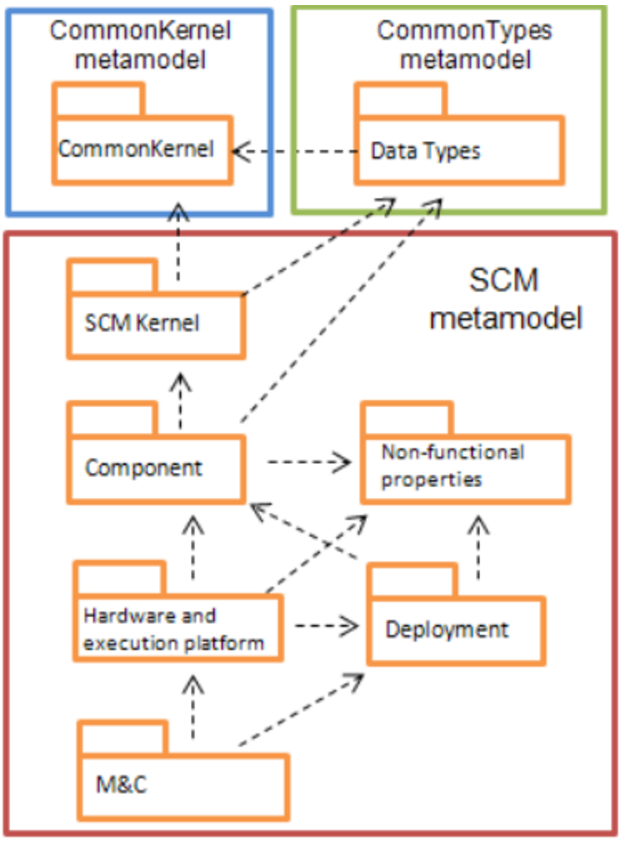
\includegraphics[width=0.4\textwidth]{LanguageUnits.pdf}
	\caption{Implementation of OSRA component model in the reference implementation}
	\source{\cite{CompBasedProcess}}
	\label{fig: Language units}
\end{figure}

\begin{description}
\item [\texttt{CommonKernel}] Defines the basic entities that are used as the base elements of the language architecture.
\item [\texttt{DataTypes}] Defines all the possible data and the data types that can be used in an OBSW model.
\item [\texttt{SCM Kernel}] Defines the infrastructural part of the \ac{scm} which can be considered as the language to express all the concerns expressed by an OBSW model.
\item [\texttt{Component}] Defines a complete set of interfacing features (interfaces, events, datasets), component types implementations and interface ports.
\item [\texttt{Non-functional properties}] Defines the non-functional properties that can be applied to the modeling entities and defines a new language called the \ac{vsl} to specify values characterized by the measurement units.
\item [\texttt{Deployment}] Defines instantiation and deployment entities such as component instances, connection between them and their deployment on the hardware architecture.
\item [\texttt{\ac{mandc}}] Defines the means to specify the technical properties related to M \& C that shall be provided in the OBSW model.
\item [\texttt{Hardware execution platform}] Defines entities related to the execution platform, \ac{tsp} and the hardware architecture.   
\end{description}

\section{OSRA SCM Model Editor}
\label{section: OSRA editor} 
The toolset that the software architect can use to build OBSW models is organized as a set of Eclipse features and Eclipse plugins \cite{OSRAEditor}. 

The toolset is available as \cite{OSRAEditor}:
\begin{itemize}
\item A pre-installed Eclipse (Eclipse Neon) for Windows 64-bit.  
\item An update site which consists of a set of static files which can be placed locally, on a web-server or on a file-server. 
\end{itemize}
In the latter case, the software architect would have to use the Eclipse Update Manager to install the plugins \cite{OSRAEditor}. 

\cref{fig: OSRA model editor} shows a screenshot of the OSRA SCM model editor.

\begin{figure}[h]
	\centering
	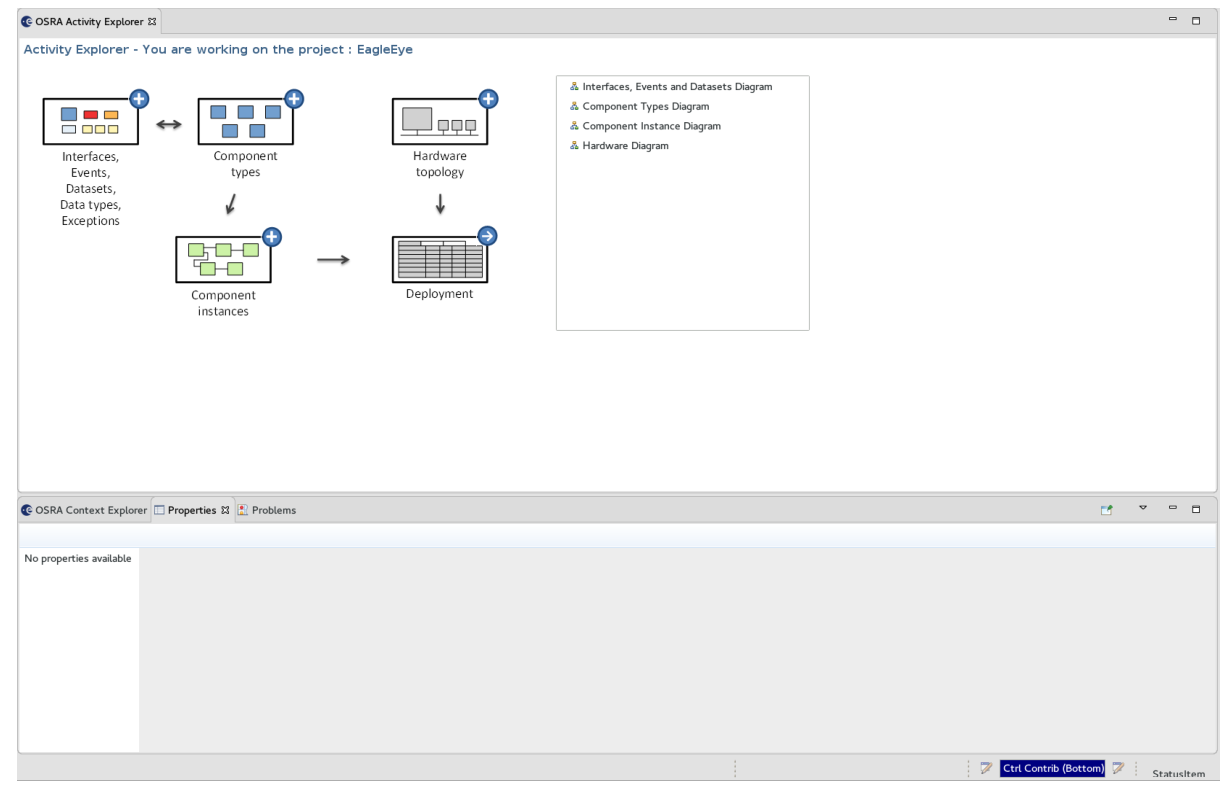
\includegraphics[width=0.8\textwidth]{OSRAModelEditor.pdf}
	\caption{Screenshot of the OSRA SCM model editor}
	\label{fig: OSRA model editor}
\end{figure}

In line with the design flow and design views explained in section \cref{section: Design flow and views}, different OSRA diagrams can be created with the help of OSRA SCM Model editor namely:
\begin{description}
\item [Interfaces, Events and Datasets diagram] This is the first diagram of the OSRA activity and allows to define the data types, events, data sets and the interfaces that would be used by the components in the Component types diagram.
\item [Component Types diagram] This is the second diagram of the OSRA activity and it allows to define the component types, device types, execution platform service types, partition proxy types, required ports whose implementation would be used by the component instances diagram.
\item [Component Instances diagram] This is the third diagram of the OSRA activity and it allows to define the component instances, device instances, execution platform service instances, partition proxy instances, provided interface slots, data receiver slots and event receiver slots.
\item [Hardware diagram] This is the last diagram of the OSRA activity and it allows to define the hardware elements such as processor boards, mass memory units, devices, buses.
\end{description}

There are also tables which are provided for diagram elements (if applicable) and they are usually found as tabs in pop-up window associated with the group that the element belongs to \cite{OSRAEditor}. Tables are one of those classical tables where rows represents an element and each column represent a potentially computed property of the element. Rows can also contain sub-rows recursively which represent the sub-elements and the software architect can collapse or expand these sub-elements as desired. More information and details about install requirements and procedure, usage of the OSRA editor can be found in \cite{OSRAEditor}.    
    

  